\documentclass[11pt,a4paper]{article}
\usepackage[T1]{fontenc}
\usepackage[utf8]{inputenc}
\usepackage{lmodern}
\usepackage{textcomp}
\usepackage[left=1.8cm,right=1.8cm,top=2.3cm,bottom=2.2cm,headheight=14pt,headsep=8pt]{geometry}
\usepackage{multicol}
\usepackage{xcolor}
\usepackage{fancyhdr}
\usepackage{graphicx}
\usepackage{array}
\usepackage{amsmath,amssymb}
\usepackage{setspace}
\usepackage{longtable}
\graphicspath{{../}}
\definecolor{ygreen}{RGB}{46,139,87}
\renewcommand{\normalsize}{\fontsize{10.9}{13.4}\selectfont}
\renewcommand{\familydefault}{\rmdefault}
\setlength{\parindent}{0pt}
\setlength{\columnsep}{0.8cm}
\setlength{\columnseprule}{0.4pt}
\setlength{\multicolsep}{3pt plus 1pt minus 1pt}
\renewcommand{\textsubscript}[1]{\ensuremath{_{\text{\fontsize{8}{8}\selectfont #1}}}}
\renewcommand{\textsuperscript}[1]{\ensuremath{^{\text{\fontsize{8}{8}\selectfont #1}}}}
\newcommand{\diqqat}[1]{\par\smallskip\noindent\textbf{Diqqat!} #1\par\medskip}
\newcommand{\javob}{\par\smallskip\noindent\textbf{Javob:} \rule[-2pt]{7.5cm}{0.4pt}\par\smallskip\noindent\textbf{Diqqat!} Javobingizni javoblar varaqasiga ko`chirib yozing.\par\medskip}
\pagestyle{fancy}
\fancyhf{}
\renewcommand{\headrulewidth}{0.4pt}
\fancyhead[L]{\textit{Milliy sertifikat 2026. Kimyo}}
\fancyhead[R]{15-variant}
\fancyfoot[L]{\fontsize{8}{9}\selectfont \textcopyright{} Colba maktabi, 2026}
\fancyfoot[C]{\thepage}
\fancypagestyle{first}{\fancyhf{}\renewcommand{\headrulewidth}{0pt}\fancyfoot[L]{\fontsize{8}{9}\selectfont \textcopyright{} Colba maktabi, 2026}\fancyfoot[C]{\thepage}}
\begin{document}
\normalsize
\thispagestyle{first}
\noindent\fcolorbox{ygreen}{white}{\parbox{\dimexpr\linewidth-2\fboxsep-2\fboxrule\relax}{%
\textbf{\fontsize{13}{15}\selectfont Nazorat testi}\ \textit{\fontsize{10}{12}\selectfont $\cdot$ Aralash test $\cdot$ 15-variant}\hfill
\begin{tabular}[t]{@{}r@{}}\textit{Milliy sertifikat 2026. Kimyo}\\ \textbf{\textit{\fontsize{8}{9}\selectfont Vaqt:}} \textit{\fontsize{10}{12}\selectfont 180 daqiqa}\end{tabular}}}
\par\medskip
\noindent\textit{Davriy jadvaldan foydalanish mumkin.}
\par\medskip
\begin{multicols}{2}
\noindent\textbf{1.} Radioaktiv izotop yadrolari sonining vaqtga bog`liqligi grafikda berilgan.
\begin{center}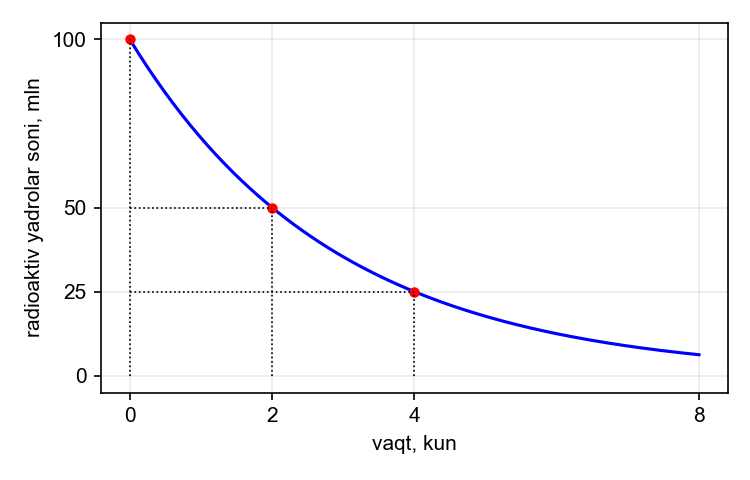
\includegraphics[width=0.86\linewidth]{rasmlar/gen/de_v15_0.png}\end{center}
4$\cdot$T vaqtdan keyin dastlabki yadrolarning necha foizi qoladi?

\noindent A)~\textsl{6,25} \hfill B)~\textsl{25} \hfill C)~\textsl{12,5} \hfill D)~\textsl{3,12}\par
\vspace{4pt}
\noindent\textbf{2.} KNO\textsubscript{3} ning suvli eritmasi inert elektrodlar bilan elektroliz qilinganda qaysi moddalar ajraladi?

\noindent\begin{tabular}{@{}p{0.47\linewidth}@{}p{0.47\linewidth}@{}}
A)~\textsl{H\textsubscript{2}, Cl\textsubscript{2} va NaOH} & B)~\textsl{Ag va O\textsubscript{2}} \\
C)~\textsl{H\textsubscript{2} va O\textsubscript{2}} & D)~\textsl{Cu va O\textsubscript{2}} \\
\end{tabular}\par
\vspace{4pt}
\noindent\textbf{3.} Tarkibida 20\% SO\textsubscript{3} bo`lgan 100 g oleum 500 g suvga qo`shildi. Hosil bo`lgan eritmadagi H\textsubscript{2}SO\textsubscript{4} ning massa \textbf{ulushini (\%) aniqlang.}

\noindent A)~\textsl{17,42} \hfill B)~\textsl{13,33} \hfill C)~\textsl{20,9} \hfill D)~\textsl{26,12}\par
\vspace{4pt}
\noindent\textbf{4.} Jadvalda bog`lar hosil qiluvchi atomlarning elektrmanfiyliklari berilgan:
\begin{center}
\renewcommand{\arraystretch}{1.15}
\begin{tabular}{|c|c|c|}\hline
\textbf{Bog`} & \textbf{EM (1-atom)} & \textbf{EM (2-atom)} \\ \hline
K--Br & 0,8 & 2,8 \\ \hline
Al--Cl & 1,5 & 3 \\ \hline
H--F & 2,1 & 4 \\ \hline
H--O & 2,1 & 3,5 \\ \hline
\end{tabular}
\end{center}
Qaysi bog` eng qutbli (eng ko`p ionli xarakterga ega)?

\noindent A)~\textsl{K--Br} \hfill B)~\textsl{Al--Cl} \hfill C)~\textsl{H--F} \hfill D)~\textsl{H--O}\par
\vspace{4pt}
\noindent\textbf{5.} 0,2 M H\textsubscript{3}PO\textsubscript{4} eritmasining normal \textbf{konsentratsiyasini (n) aniqlang.}

\noindent A)~\textsl{0,2} \hfill B)~\textsl{1,2} \hfill C)~\textsl{0,6} \hfill D)~\textsl{0,067}\par
\vspace{4pt}
\noindent\textbf{6.} Jadvalda metall plastinkalarning tuz eritmalariga tushirilishidagi kuzatuvlar berilgan (``+'' -- metall ajraladi, reaksiya boradi; ``$-$'' -- reaksiya bormaydi):
\begin{center}
\renewcommand{\arraystretch}{1.15}
\begin{tabular}{|c|c|c|c|}\hline
\textbf{Metall} & \textbf{FeSO\textsubscript{4} eritmasi} & \textbf{ZnSO\textsubscript{4} eritmasi} & \textbf{MgSO\textsubscript{4} eritmasi} \\ \hline
Fe & $-$ & $-$ & $-$ \\ \hline
Mg & + & + & $-$ \\ \hline
Ag & $-$ & $-$ & $-$ \\ \hline
\end{tabular}
\end{center}
Ushbu metallardan qaysi biri eng faol?

\noindent A)~\textsl{Fe} \hfill B)~\textsl{Ag} \hfill C)~\textsl{Zn} \hfill D)~\textsl{Mg}\par
\vspace{4pt}
\noindent\textbf{7.} 4 g NaOH ni to`liq neytrallash uchun 6 g CH\textsubscript{3}COOH sarflandi. CH\textsubscript{3}COOH ning ekvivalent \textbf{massasini (g/mol) aniqlang.}

\noindent A)~\textsl{120} \hfill B)~\textsl{60} \hfill C)~\textsl{30} \hfill D)~\textsl{6}\par
\vspace{4pt}
\noindent\textbf{8.} 2 mol Ba(OH)\textsubscript{2} va 3 mol AlCl\textsubscript{3} suvda eritilib, eritma hajmi 4 l ga yetkazildi. Eritmadagi barcha ionlarning umumiy molyar \textbf{konsentratsiyasini (mol/l) aniqlang} (kuchli elektrolitlar to`liq dissotsilanadi).

\noindent A)~\textsl{1,25} \hfill B)~\textsl{9} \hfill C)~\textsl{2,25} \hfill D)~\textsl{4,5}\par
\vspace{4pt}
\noindent\textbf{9.} Quyidagi zarrachalardan qaysilari neon atomi bilan izoelektron? 1) O\textsuperscript{2$-$}; 2) F\textsuperscript{$-$}; 3) Cl\textsuperscript{$-$}; 4) K\textsuperscript{+}

\noindent A)~\textsl{2, 3, 4} \hfill B)~\textsl{1, 2} \hfill C)~\textsl{3, 4} \hfill D)~\textsl{1, 2, 4}\par
\vspace{4pt}
\noindent\textbf{10.} Mis atomida d-pog`onachadagi elektronlar \textbf{sonini aniqlang} (\textit{Z} = 29).

\noindent A)~\textsl{11} \hfill B)~\textsl{9} \hfill C)~\textsl{12} \hfill D)~\textsl{10}\par
\vspace{4pt}
\end{multicols}
\noindent\textbf{11.} K\textsubscript{2}Cr\textsubscript{2}O\textsubscript{7} tuzining eruvchanligi (g/100 g suv) haroratga bog`liq jadvalda keltirilgan:
\begin{center}
\renewcommand{\arraystretch}{1.15}
\begin{tabular}{|c|c|c|c|c|}\hline
\textbf{t, \textdegree{}C} & \textbf{0} & \textbf{20} & \textbf{40} & \textbf{60} \\ \hline
S, g/100 g suv & 15 & 24 & 38 & 60 \\ \hline
\end{tabular}
\end{center}
60 \textdegree{}C da tayyorlangan to`yingan 480 g eritma 20 \textdegree{}C gacha sovitildi. Cho`kmaga tushgan tuz \textbf{massasini (g) aniqlang.}

\noindent A)~\textsl{180} \hfill B)~\textsl{72} \hfill C)~\textsl{108} \hfill D)~\textsl{216}\par
\vspace{4pt}
\begin{multicols}{2}
\noindent\textbf{12.} 32,2 g Na\textsubscript{2}SO\textsubscript{4}$\cdot$10H\textsubscript{2}O 300 g suvda eritildi. Eritmadagi tuzning massa \textbf{ulushini (\%) aniqlang.}

\noindent A)~\textsl{4,73} \hfill B)~\textsl{9,69} \hfill C)~\textsl{4,27} \hfill D)~\textsl{8,55}\par
\vspace{4pt}
\noindent\textbf{13.} Faqat qaytaruvchi bo`la oladigan \textbf{ionlarni aniqlang}: 1) Fe\textsuperscript{2+}; 2) Ag\textsuperscript{+}; 3) Cl\textsuperscript{$-$}; 4) Na\textsuperscript{+}

\noindent A)~\textsl{4} \hfill B)~\textsl{3} \hfill C)~\textsl{3, 4} \hfill D)~\textsl{1, 4}\par
\vspace{4pt}
\noindent\textbf{14.} D-metallar va ularning birikmalari haqida qaysi fikrlar to`g`ri? 1) Fe(OH)\textsubscript{2} havoda qo`ng`ir rangga o`tadi; 2) Xrom (VI) oksidi (CrO\textsubscript{3}) kislotali oksid; 3) Cu(OH)\textsubscript{2} qizdirilganda CuO ga parchalanadi; 4) Temir sovuq konsentrlangan HNO\textsubscript{3} da passivlanadi

\noindent\begin{tabular}{@{}p{0.47\linewidth}@{}p{0.47\linewidth}@{}}
A)~\textsl{2, 3, 4} & B)~\textsl{1, 2, 4} \\
C)~\textsl{1, 3, 4} & D)~\textsl{1, 2, 3, 4} \\
\end{tabular}\par
\vspace{4pt}
\noindent\textbf{15.} Rasmda metallarning kuchlanish qatori ko`rsatilgan (\textit{X}, \textit{Y}, \textit{Z} --- noma'lum metallar).
\begin{center}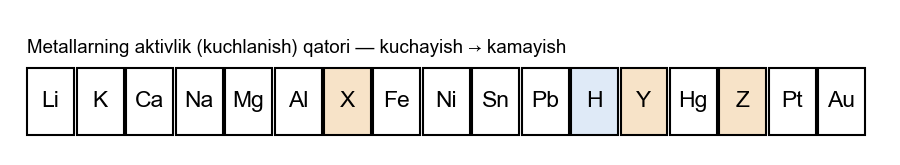
\includegraphics[width=0.86\linewidth]{rasmlar/gen/se_696275.png}\end{center}
\textit{X} metali tuzining eritmasiga \textit{Y} metall plastinka tushirilsa, reaksiya boradimi?
\noindent A)~\textsl{Bormaydi, \textit{Y} kamroq faol}\par
\noindent B)~\textsl{Boradi, \textit{Y} faolroq}\par
\noindent C)~\textsl{Faqat qizdirilganda boradi}\par
\noindent D)~\textsl{Faqat konsentrlangan eritmada boradi}\par
\vspace{4pt}
\noindent\textbf{16.} SO\textsubscript{3} + 2KOH $\to$ K\textsubscript{2}SO\textsubscript{4} + H\textsubscript{2}O jarayoni uchun 80 g SO\textsubscript{3} olingan (unum 90\%). KOH \textbf{massasini (g) aniqlang.}

\noindent A)~\textsl{28} \hfill B)~\textsl{201,6} \hfill C)~\textsl{100,8} \hfill D)~\textsl{50,4}\par
\vspace{4pt}
\noindent\textbf{17.} BaCl\textsubscript{2} + Na\textsubscript{2}SO\textsubscript{4} $\to$ BaSO\textsubscript{4} + 2NaCl reaksiyasida tarkibida 20\% aralashma bo`lgan 260 g namuna (asosiy modda BaCl\textsubscript{2}) ishtirok etdi. BaSO\textsubscript{4} \textbf{massasini (g) toping.}

\noindent A)~\textsl{233} \hfill B)~\textsl{466} \hfill C)~\textsl{116,5} \hfill D)~\textsl{349,5}\par
\vspace{4pt}
\noindent\textbf{18.} Quyidagi mineral o`g`itlardan qaysilari fosforli o`g`itlar jumlasiga kiradi? 1) Ca(H\textsubscript{2}PO\textsubscript{4})\textsubscript{2}; 2) Ca\textsubscript{3}(PO\textsubscript{4})\textsubscript{2}; 3) K\textsubscript{2}SO\textsubscript{4}; 4) (NH\textsubscript{4})\textsubscript{2}HPO\textsubscript{4}

\noindent A)~\textsl{3, 4} \hfill B)~\textsl{1, 4} \hfill C)~\textsl{2, 3} \hfill D)~\textsl{1, 2}\par
\vspace{4pt}
\noindent\textbf{19.} Reaksiya tenglamasi: 2NaNO\textsubscript{3} $\to$ 2NaNO\textsubscript{2} + O\textsubscript{2}. Reaksiyaga 17 g NaNO\textsubscript{3} kirishdi. NaNO\textsubscript{2} \textbf{massasini (g) hisoblang.}

\noindent A)~\textsl{13,8} \hfill B)~\textsl{27,6} \hfill C)~\textsl{6,9} \hfill D)~\textsl{20,7}\par
\vspace{4pt}
\noindent\textbf{20.} 30 g C\textsubscript{2}H\textsubscript{6} dan quyidagi ikki bosqichda KCl olinadi: 1) C\textsubscript{2}H\textsubscript{6} + Cl\textsubscript{2} $\to$ C\textsubscript{2}H\textsubscript{5}Cl + HCl (unum 90\%); 2) C\textsubscript{2}H\textsubscript{5}Cl + KOH $\to$ C\textsubscript{2}H\textsubscript{5}OH + KCl (unum 90\%). Oxirgi mahsulot KCl ning \textbf{massasini (g) toping.}

\noindent A)~\textsl{67,05} \hfill B)~\textsl{74,5} \hfill C)~\textsl{120,69} \hfill D)~\textsl{60,35}\par
\vspace{4pt}
\noindent\textbf{21.} Alken, alkadiyen va alkinlar haqida qaysi fikrlar to`g`ri? 1) Asetilen Ag\textsubscript{2}O ning ammiakli eritmasi bilan cho`kma beradi (butin-2 beradi); 2) Etilen bromli suvni rangsizlantiradi; 3) Alkenlar KMnO\textsubscript{4} ning suvli eritmasi bilan glikol hosil qiladi; 4) Etilen sanoatda kreking gazlaridan olinadi

\noindent A)~\textsl{1, 4} \hfill B)~\textsl{2, 3, 4} \hfill C)~\textsl{2, 3} \hfill D)~\textsl{3, 4}\par
\vspace{4pt}
\noindent\textbf{22.} Arenlar, neft va tabiiy gaz haqida qaysi fikrlar to`g`ri? 1) Benzoldan nitrobenzol nitrolash bilan olinadi; 2) Benzolda 6 ta sp\textsuperscript{2} gibridlangan uglerod bor; 3) Neft fraksiyalaridan gazolin 150 \textdegree{}C gacha haydaladi; 4) Toluol KMnO\textsubscript{4} bilan benzoy kislotagacha oksidlanadi

\noindent\begin{tabular}{@{}p{0.47\linewidth}@{}p{0.47\linewidth}@{}}
A)~\textsl{1, 2, 3} & B)~\textsl{1, 2, 3, 4} \\
C)~\textsl{2, 3, 4} & D)~\textsl{1, 3, 4} \\
\end{tabular}\par
\vspace{4pt}
\noindent\textbf{23.} CH\textsubscript{3}OH va C\textsubscript{3}H\textsubscript{7}OH dan iborat 12,4 g aralashma natriy bilan to`liq reaksiyaga kirishganda ajraladigan vodorod \textbf{hajmini (l, n.sh.) toping.}

\noindent A)~\textsl{6,72} \hfill B)~\textsl{1,68} \hfill C)~\textsl{3,36} \hfill D)~\textsl{1,51}\par
\vspace{4pt}
\noindent\textbf{24.} Aldegid va ketonlar haqida qaysi fikrlar to`g`ri? 1) Sirka aldegid Kucherov reaksiyasi bilan olinadi; 2) Aldegidlar qaytarilganda ikkilamchi spirt hosil bo`ladi; 3) Ketonlar kuchsiz oksidlovchilar bilan oksidlanmaydi; 4) Formaldegid gaz holatda, suvda yaxshi eriydi

\noindent A)~\textsl{1, 4} \hfill B)~\textsl{1, 2} \hfill C)~\textsl{2, 3} \hfill D)~\textsl{1, 3, 4}\par
\vspace{4pt}
\noindent\textbf{25.} 30 g CH\textsubscript{3}COOH dan quyidagi ikki bosqichda Na\textsubscript{2}CO\textsubscript{3} olinadi: 1) CH\textsubscript{3}COOH + NaHCO\textsubscript{3} $\to$ CH\textsubscript{3}COONa + CO\textsubscript{2} + H\textsubscript{2}O (unum 80\%); 2) CH\textsubscript{3}COONa + NaOH $\to$ CH\textsubscript{4} + Na\textsubscript{2}CO\textsubscript{3} (unum 50\%). Oxirgi mahsulot Na\textsubscript{2}CO\textsubscript{3} ning \textbf{massasini (g) toping.}

\noindent A)~\textsl{26,5} \hfill B)~\textsl{21,2} \hfill C)~\textsl{42,4} \hfill D)~\textsl{53}\par
\vspace{4pt}
\noindent\textbf{26.} 89 g tristearin natriy ishqori bilan to`liq gidrolizlanganda necha gramm sovun hosil bo`ladi?

\noindent A)~\textsl{30,6} \hfill B)~\textsl{91,8} \hfill C)~\textsl{61,2} \hfill D)~\textsl{89}\par
\vspace{4pt}
\noindent\textbf{27.} Quyidagi birikmalardan qaysi biri spirt sinfiga kiradi?

\noindent A)~\textsl{CH\textsubscript{3}CHO} \hfill B)~\textsl{C\textsubscript{2}H\textsubscript{5}NH\textsubscript{2}} \hfill C)~\textsl{C\textsubscript{2}H\textsubscript{5}OH} \hfill D)~\textsl{CH\textsubscript{3}OCH\textsubscript{3}}\par
\vspace{4pt}
\noindent\textbf{28.} Aminlar, aminokislotalar va oqsillar haqida qaysi fikrlar to`g`ri? 1) Glitsin optik faol; 2) Aminokislotalar faqat kislotali xossaga ega; 3) Aminokislotalar amfoter birikmalar; 4) Dipeptidda 2 ta peptid bog` bor

\noindent A)~\textsl{3} \hfill B)~\textsl{1} \hfill C)~\textsl{2, 3} \hfill D)~\textsl{1, 2}\par
\vspace{4pt}
\noindent\textbf{29.} 5,2 g C\textsubscript{2}H\textsubscript{2} dan quyidagi ikki bosqichda C\textsubscript{2}H\textsubscript{6} olinadi: 1) C\textsubscript{2}H\textsubscript{2} + H\textsubscript{2} $\to$ C\textsubscript{2}H\textsubscript{4} (unum 60\%); 2) C\textsubscript{2}H\textsubscript{4} + H\textsubscript{2} $\to$ C\textsubscript{2}H\textsubscript{6} (unum 50\%). Oxirgi mahsulot C\textsubscript{2}H\textsubscript{6} ning \textbf{hajmini (l, n.sh.) toping.}

\noindent A)~\textsl{1,34} \hfill B)~\textsl{2,24} \hfill C)~\textsl{2,69} \hfill D)~\textsl{4,48}\par
\vspace{4pt}
\noindent\textbf{30.} 400 g 5\% li Na\textsubscript{2}CO\textsubscript{3} eritmasini Na\textsubscript{2}CO\textsubscript{3}$\cdot$10H\textsubscript{2}O dan tayyorlash uchun necha gramm kristallogidrat kerak?

\noindent A)~\textsl{20} \hfill B)~\textsl{107,92} \hfill C)~\textsl{53,96} \hfill D)~\textsl{26,98}\par
\vspace{4pt}
\noindent\textbf{31.} KNO\textsubscript{3} ning 50\% li eritmasidan 200 g 8\% li eritma tayyorlash uchun necha gramm suv kerak?

\noindent A)~\textsl{32} \hfill B)~\textsl{168} \hfill C)~\textsl{200} \hfill D)~\textsl{336}\par
\vspace{4pt}
\noindent\textbf{32.} Rasmdagi asbobda CO\textsubscript{2} olish uchun qaysi moddalar ishlatilgan?
\begin{center}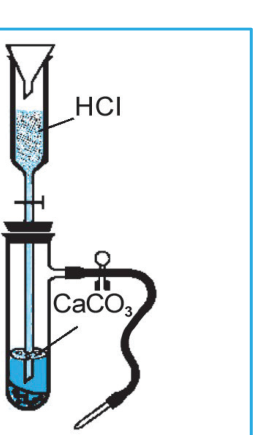
\includegraphics[width=0.86\linewidth]{rasmlar/darslik/d_co2.png}\end{center}

\noindent\begin{tabular}{@{}p{0.47\linewidth}@{}p{0.47\linewidth}@{}}
A)~\textsl{NH\textsubscript{4}Cl va Ca(OH)\textsubscript{2}} & B)~\textsl{Zn va HCl} \\
C)~\textsl{NaCl va H\textsubscript{2}SO\textsubscript{4}} & D)~\textsl{CaCO\textsubscript{3} va HCl   ---} \\
\end{tabular}\par
\vspace{4pt}
\end{multicols}
\medskip
\noindent\setlength{\fboxsep}{0pt}\fbox{\begin{tabular}{p{0.74\linewidth}|p{0.2\linewidth}}
\parbox[t]{0.72\linewidth}{\vspace{3pt}\textbf{Topshiriqlar (33--35) va javob variant (A--F)larini o`zaro to`g`ri moslashtiring.} Na va Na\textsubscript{2}O dan iborat 17 g aralashma 200 g suvda to`liq eritildi, bunda 2,24 l (n.sh.) vodorod ajraldi. Hosil bo`lgan eritma sirka kislota bilan to`liq neytrallandi.
\vspace{3pt}} & \parbox[t]{0.19\linewidth}{\vspace{3pt}A~\textsl{180}\\[3pt]
B~\textsl{24,8}\\[3pt]
C~\textsl{11,07}\\[3pt]
D~\textsl{90}\\[3pt]
E~\textsl{12,4}\\[3pt]
F~\textsl{18,6}}\\ \hline
\parbox[t]{0.72\linewidth}{\vspace{2pt}\textbf{33. Hosil bo`lgan eritmadagi NaOH ning massa ulushini (\%) aniqlang.}\vspace{2pt}} & \\ \hline
\parbox[t]{0.72\linewidth}{\vspace{2pt}\textbf{34. Dastlabki aralashmadagi Na\textsubscript{2}O massasini (g) aniqlang.}\vspace{2pt}} & \\ \hline
\parbox[t]{0.72\linewidth}{\vspace{2pt}\textbf{35. Neytrallash uchun sarflangan 20\% li sirka kislota eritmasining massasini (g) aniqlang.}\vspace{2pt}} & 
\end{tabular}}
\par\bigskip
\noindent\textbf{36.} K\textsubscript{2}Cr\textsubscript{2}O\textsubscript{7} + KI + H\textsubscript{2}SO\textsubscript{4} $\to$ Cr\textsubscript{2}(SO\textsubscript{4})\textsubscript{3} + I\textsubscript{2} + K\textsubscript{2}SO\textsubscript{4} + H\textsubscript{2}O reaksiya tenglamasini tenglang. Reagentlar (chap qism) koeffitsiyentlari \textbf{yig`indisini toping.}
\javob
\noindent\textbf{37.} 10 g CaCO\textsubscript{3} reaksiyaga kirishdi (CaCO\textsubscript{3} + 2HCl $\to$ CaCl\textsubscript{2} + CO\textsubscript{2} + H\textsubscript{2}O). Ajralgan CO\textsubscript{2} \textbf{hajmini (l, n.sh.) hisoblang} (unum 80\%).
\javob
\noindent\textbf{38.} 100 m\textsuperscript{3} suvda Ca(HCO\textsubscript{3})\textsubscript{2} konsentratsiyasi 20 mol/m\textsuperscript{3}, Mg(HCO\textsubscript{3})\textsubscript{2} niki 20 mol/m\textsuperscript{3}. Suvni Ca(OH)\textsubscript{2} bilan to`liq yumshatish uchun Ca(OH)\textsubscript{2} ning \textbf{massasini (kg) hisoblang.}
\javob
\noindent\textbf{39.} 90 g glyukoza spirtli bijg`ish natijasida etanolga (unum 90\%), hosil bo`lgan etanol esa sirka kislotagacha (unum 80\%) aylantirildi. Olingan kislotani to`liq neytrallash uchun NaOH ning \textbf{massasini (g) toping.}
\javob
\noindent\textbf{40.} 7,4 g CH\textsubscript{3}COOCH\textsubscript{3} mo`l NaOH bilan to`liq gidrolizlandi. Hosil bo`lgan tuz \textbf{massasini (g) aniqlang.}
\javob
\par\bigskip\begin{center}\textbf{\fontsize{13}{15}\selectfont YOZMA ISH}\end{center}
\noindent\textbf{41.} \textbf{Topshiriqni bajarish jarayonida barcha reaksiya tenglamalarini yozing. Miqdoriy va arifmetik hisoblashlarni (unga asos bo`lgan usul yoki formulani ko`rsatgan holda) uzviy ketma-ketlikda bajaring.}\par\smallskip
Laboratoriyada xlor olish uchun MnO\textsubscript{2} ga konsentrlangan xlorid kislota ta'sir ettirildi: MnO\textsubscript{2} + 4HCl $\to$ MnCl\textsubscript{2} + Cl\textsubscript{2} + 2H\textsubscript{2}O. Ajralgan 13,44 l (n.sh.) xlor gazining yarmi mo`l KI eritmasidan o`tkazildi, qolgan yarmi esa issiq mo`l KOH eritmasiga yuttirildi.\par
\noindent 1)Reaksiyani elektron balans usulida tenglang: oksidlovchi va qaytaruvchini ko`rsating, koeffitsiyentlar yig`indisini toping.\par
\noindent 2)MnO\textsubscript{2} ning sarflangan massasini (g) hisoblang. Sarflangan oksidlovchining miqdorini (mol) ham toping.\par
\noindent 3)Sarflangan HCl miqdorini (mol) va shundan qaytaruvchi sifatida ishtirok etgan qismini (mol) aniqlang.\par
\noindent 4)Xlor mo`l KI eritmasidan o`tkazilganda ajralgan yodning massasini (g) toping (reaksiya tenglamasini yozing). Sarflangan KI massasini (g) ham toping.\par
\noindent 5)Issiq KOH eritmasiga yuttirilganda (3Cl\textsubscript{2} + 6KOH $\to$ KClO\textsubscript{3} + 5KCl + 3H\textsubscript{2}O) hosil bo`lgan KClO\textsubscript{3} massasini (g) aniqlang. Agar xlor sovuq KOH eritmasiga yuttirilsa (Cl\textsubscript{2} + 2KOH $\to$ KCl + KClO + H\textsubscript{2}O), hosil bo`ladigan KClO massasini (g) ham toping.\par
\diqqat{Mazkur topshiriq kengaytirilgan javobni talab etib, uning yechilish usuli va shu usul asosidagi barcha hisoblash amallari javoblar varaqasida aks etishi lozim.}
\noindent\textbf{42.} Quyidagi o`zgarishlar zanjirida \textit{X}, \textit{Y}, \textit{Z} noma'lum organik moddalar:\par
\[\setlength{\fboxsep}{0pt}\text{CH\textsubscript{3}CHO}\xrightarrow{\text{Ag\textsubscript{2}O, NH\textsubscript{3}}}\text{\textit{X}}\xrightarrow{\text{C\textsubscript{2}H\textsubscript{5}OH, H\textsubscript{2}SO\textsubscript{4}}}\text{\textit{Y}}\xrightarrow{\text{NaOH}}\text{\textit{Z}}\xrightarrow{\text{NaOH (suyuqlanma), t\textdegree{}}}\text{CH\textsubscript{4}}\]
\noindent 1)CH\textsubscript{3}CHO $\to$ \textit{X} : reaksiya tenglamasini yozing; hosil bo`lgan moddani nomlang.\par
\noindent 2)\textit{X} $\to$ \textit{Y} : reaksiya tenglamasini yozing; hosil bo`lgan moddani nomlang.\par
\noindent 3)\textit{Y} $\to$ \textit{Z} : reaksiya tenglamasini yozing; hosil bo`lgan moddani nomlang.\par
\noindent 4)\textit{Z} $\to$ CH\textsubscript{4} : reaksiya tenglamasini yozing; hosil bo`lgan moddani nomlang.\par
\diqqat{Mazkur topshiriq kengaytirilgan javobni talab etib, uning yechilish usuli va shu usul asosidagi barcha hisoblash amallari javoblar varaqasida aks etishi lozim.}
\noindent\textbf{43.} \textbf{Topshiriqni bajarish jarayonida barcha reaksiya tenglamalarini yozing. Miqdoriy va arifmetik hisoblashlarni (unga asos bo`lgan usul yoki formulani ko`rsatgan holda) uzviy ketma-ketlikda bajaring.}\par\smallskip
CaCO\textsubscript{3} va MgCO\textsubscript{3} dan iborat 36,8 g aralashma doimiy massagacha qizdirildi. Ajralgan gaz mo`l Ca(OH)\textsubscript{2} eritmasidan o`tkazildi.\par
\noindent 1)Aralashmadagi har bir tuzning massasini (g) va massa ulushini (\%) aniqlang (reaksiya tenglamalarini yozing).\par
\noindent 2)Ajralgan gaz hajmini (l, n.sh.) va qattiq qoldiq massasini (g) toping. Qoldiqdagi CaO ning massa ulushini (\%) ham hisoblang.\par
\noindent 3)Gaz Ca(OH)\textsubscript{2} eritmasidan o`tkazilganda hosil bo`lgan cho`kma massasini (g) hisoblang.\par
\noindent 4)Qattiq qoldiqni to`liq eritish uchun 10\% li HCl eritmasidan necha gramm kerak?\par
\noindent 5)Qoldiq oksidlar suvga solinganda hosil bo`ladigan Ca(OH)\textsubscript{2} massasini (g) toping (CaO + H\textsubscript{2}O $\to$ Ca(OH)\textsubscript{2}).\par
\diqqat{Mazkur topshiriq kengaytirilgan javobni talab etib, uning yechilish usuli va shu usul asosidagi barcha hisoblash amallari javoblar varaqasida aks etishi lozim.}
\newpage
\noindent\textbf{\fontsize{13}{15}\selectfont Nazorat testi}\ \textit{$\cdot$ 15-variant}\hfill \textbf{Javoblar kaliti}\par\smallskip\hrule\smallskip
\textit{Faqat o`qituvchi uchun.}\par\medskip
\noindent\textbf{1--32-savollar}\par\smallskip
\noindent\begin{tabular}{|c|c|c|c|c|c|c|c|c|c|c|c|c|c|c|c|}\hline
\textbf{1} & \textbf{2} & \textbf{3} & \textbf{4} & \textbf{5} & \textbf{6} & \textbf{7} & \textbf{8} & \textbf{9} & \textbf{10} & \textbf{11} & \textbf{12} & \textbf{13} & \textbf{14} & \textbf{15} & \textbf{16}\\\hline
\textsl{A} & \textsl{C} & \textsl{A} & \textsl{A} & \textsl{C} & \textsl{D} & \textsl{B} & \textsl{D} & \textsl{B} & \textsl{D} & \textsl{C} & \textsl{C} & \textsl{B} & \textsl{D} & \textsl{A} & \textsl{C}\\\hline
\textbf{17} & \textbf{18} & \textbf{19} & \textbf{20} & \textbf{21} & \textbf{22} & \textbf{23} & \textbf{24} & \textbf{25} & \textbf{26} & \textbf{27} & \textbf{28} & \textbf{29} & \textbf{30} & \textbf{31} & \textbf{32}\\\hline
\textsl{A} & \textsl{D} & \textsl{A} & \textsl{D} & \textsl{B} & \textsl{B} & \textsl{C} & \textsl{D} & \textsl{B} & \textsl{B} & \textsl{C} & \textsl{A} & \textsl{A} & \textsl{C} & \textsl{B} & \textsl{D}\\\hline
\end{tabular}\par\medskip
\noindent\textbf{33--35-savollar}\par\smallskip
\noindent\begin{tabular}{|c|c|c|}\hline \textbf{No} & \textbf{Javob} & \textbf{Qiymat}\\\hline
33 & \textsl{C} & 11,07\\\hline
34 & \textsl{E} & 12,4\\\hline
35 & \textsl{A} & 180\\\hline
\end{tabular}\par\medskip
\noindent\textbf{36--40-savollar}\par\smallskip
\noindent\begin{tabular}{|c|c|}\hline \textbf{No} & \textbf{To`g`ri javob}\\\hline
36 & 14\\\hline
37 & 1,79\\\hline
38 & 444\\\hline
39 & 28,8\\\hline
40 & 8,2\\\hline
\end{tabular}\par\medskip
\noindent\textbf{41--43-topshiriqlar: qisqa yechim}\par\smallskip
\noindent\textbf{41-topshiriq.}\par
\noindent 1) Tenglama: MnO\textsubscript{2} + 4HCl $\to$ MnCl\textsubscript{2} + Cl\textsubscript{2} + 2H\textsubscript{2}O; oksidlovchi MnO\textsubscript{2}, qaytaruvchi Cl\textsuperscript{$-$} (HCl); koeffitsiyentlar yig`indisi \textbf{9}\par
\noindent 2) n(Cl\textsubscript{2}) = 0,6 mol; n(MnO\textsubscript{2}) = 0,6$\cdot$1/1 = 0,6 mol $\to$ m = \textbf{52,2 g}; n(MnO\textsubscript{2}) = \textbf{0,6 mol}\par
\noindent 3) n(HCl) = 2,4 mol (\textbf{2,4 mol}); qaytaruvchi: \textbf{1,2 mol}\par
\noindent 4) Cl\textsubscript{2} + 2KI $\to$ 2KCl + I\textsubscript{2}: n(Cl\textsubscript{2}) = 0,3 mol $\to$ n(I\textsubscript{2}) = 0,3 mol $\to$ \textbf{76,2 g}; n(KI) = 2$\cdot$0,3 = 0,6 mol $\to$ \textbf{99,6 g}\par
\noindent 5) n(Cl\textsubscript{2}) = 0,3 mol; n(KClO\textsubscript{3}) = 0,3/3 = 0,1 mol $\to$ \textbf{12,25 g}; n(KClO) = 0,3 mol $\to$ \textbf{22,35 g}\par
\noindent Jami: M 15 + A 10 = 25 ball.\par
\noindent\textbf{42-topshiriq.}\par
\noindent 1) CH\textsubscript{3}CHO + Ag\textsubscript{2}O, NH\textsubscript{3} $\to$ CH\textsubscript{3}COOH (sirka kislota)\par
\noindent 2) CH\textsubscript{3}COOH + C\textsubscript{2}H\textsubscript{5}OH, H\textsubscript{2}SO\textsubscript{4} $\to$ CH\textsubscript{3}COOC\textsubscript{2}H\textsubscript{5} (etilatsetat)\par
\noindent 3) CH\textsubscript{3}COOC\textsubscript{2}H\textsubscript{5} + NaOH $\to$ CH\textsubscript{3}COONa (natriy atsetat)\par
\noindent 4) CH\textsubscript{3}COONa + NaOH (suyuqlanma), t\textdegree{} $\to$ CH\textsubscript{4} (metan)\par
\noindent Jami 25 ball.\par
\noindent\textbf{43-topshiriq.}\par
\noindent 1) x$\cdot$100 + y$\cdot$84 = 36,8; x + y = 0,4 $\to$ CaCO\textsubscript{3} 20 g (54,3\%), MgCO\textsubscript{3} 16,8 g (45,7\%)\par
\noindent 2) n(CO\textsubscript{2}) = 0,4 mol $\to$ \textbf{8,96 l}; qoldiq CaO + MgO = \textbf{19,2 g}; $\omega$(CaO) = 11,2/19,2 = \textbf{58,3\%}\par
\noindent 3) CO\textsubscript{2} + Ca(OH)\textsubscript{2} $\to$ CaCO\textsubscript{3}$\downarrow$ + H\textsubscript{2}O: 0,4 mol $\to$ \textbf{40 g}\par
\noindent 4) CaO + 2HCl; MgO + 2HCl: n(HCl) = 0,8 mol = 29,2 g $\to$ 10\% li eritma \textbf{292 g}\par
\noindent 5) n(CaO) = 0,2 mol $\to$ m(Ca(OH)\textsubscript{2}) = 0,2$\cdot$74 = \textbf{14,8 g}\par
\noindent Jami: M 15 + A 10 = 25 ball.\par
\par\bigskip\noindent\textbf{Mavzular taqsimoti}\par\smallskip
{\small\noindent\begin{longtable}{|c|p{7.2cm}|p{5.4cm}|c|}\hline \textbf{No} & \textbf{Mavzu} & \textbf{Tekshiriladigan ko`nikma} & \textbf{Ball}\\\hline
1 & 11-sinf (yadro) & Grafik tahlili & 1\\\hline
2 & 11-sinf 8-bob; Tirkashev \textit{V} bob (elektroliz) & Bilim va tushunish & 1\\\hline
3 & Tirkashev III bob (oleum); Tashev & Hisoblash va masala yechish & 1\\\hline
4 & 8-sinf (kimyoviy bog`lanish turlari, jadval) & Jadval tahlili & 1\\\hline
5 & 11-sinf 4-bob (normal konsentratsiya) & Hisoblash va masala yechish & 1\\\hline
6 & Tirkashev \textit{V} bob (kuchlanish qatori, jadval) & Jadval tahlili & 1\\\hline
7 & 11-sinf (ekvivalentlar qonuni) & Hisoblash va masala yechish & 1\\\hline
8 & Tirkashev IV bob (kuchli elektrolitlar) & Hisoblash va masala yechish & 1\\\hline
9 & Tirkashev I bob; 8-sinf (izoelektron) & Bilim va tushunish & 1\\\hline
10 & Tirkashev I bob; 8-sinf (elektron konfiguratsiya) & Bilim va tushunish & 1\\\hline
11 & Tirkashev III bob (eruvchanlik, jadval) & Jadval tahlili & 1\\\hline
12 & Tirkashev III bob (kristallogidrat) & Hisoblash va masala yechish & 1\\\hline
13 & Tirkashev \textit{V} bob; 11-sinf 7-bob & Bilim va tushunish & 1\\\hline
14 & 9-sinf; Tashev (Fe, Cu, Zn, Cr) & Bilim va tushunish & 1\\\hline
15 & 9-sinf (metallar aktivligi) & Rasm bo`yicha tahlil & 1\\\hline
16 & 9-sinf; Tirkashev (oksid/asos/kislota/tuz, hisob) & Hisoblash va masala yechish & 1\\\hline
17 & 9-sinf; Tirkashev (genetik zanjir/reaksiya turlari, hisob) & Hisoblash va masala yechish & 1\\\hline
18 & Tashev (mineral o`g`itlar) & Bilim va tushunish & 1\\\hline
19 & 9-sinf; Tirkashev (tuzlarning termik parchalanishi, hisob) & Hisoblash va masala yechish & 1\\\hline
20 & 10-sinf (ikki bosqichli hisob) & Hisoblash va masala yechish & 1\\\hline
21 & 10-sinf (mavzuga oid paragraflar); Abdusamatov & Bilim va tushunish & 1\\\hline
22 & 10-sinf (mavzuga oid paragraflar); Abdusamatov & Bilim va tushunish & 1\\\hline
23 & 10-sinf \S{}21 (spirtlar) & Hisoblash va masala yechish & 1\\\hline
24 & 10-sinf (mavzuga oid paragraflar); Abdusamatov & Bilim va tushunish & 1\\\hline
25 & 10-sinf (ikki bosqichli hisob) & Hisoblash va masala yechish & 1\\\hline
26 & 10-sinf \S{}29 (yog`lar, sovunlanish) & Hisoblash va masala yechish & 1\\\hline
27 & 10-sinf (organik birikmalar sinflari) & Bilim va tushunish & 1\\\hline
28 & 10-sinf (mavzuga oid paragraflar); Abdusamatov & Bilim va tushunish & 1\\\hline
29 & 10-sinf (ikki bosqichli hisob) & Hisoblash va masala yechish & 1\\\hline
30 & Tirkashev III bob; 7-sinf (eritma tayyorlash) & Hisoblash va masala yechish & 1\\\hline
31 & Tirkashev III bob (eritmalar) & Hisoblash va masala yechish & 1\\\hline
32 & 9-sinf (11-rasm) & Rasm bo`yicha tahlil & 1\\\hline
33--35 & Aralash masala (moslashtirish) & Ko`p bosqichli hisob & 3\\\hline
36--40 & Qisqa javobli masalalar & Hisoblash & 5\\\hline
41--43 & Yozma ish & Usul va hisob (M, A) & 75\\\hline
\end{longtable}}
\end{document}
